\clearpage
% \newpage
\setcounter{page}{1}


\twocolumn[{
\renewcommand\twocolumn[1][]{#1}
\section{Case Study and Evaluation}
We present cases generated by M-DocSum-7B and Qwen2-VL-7B in Figure~\ref{fig:case_en_2} and Figure~\ref{fig:case_en_1}, and elaborate on the calculation methods of the M-DocEval metrics.


% \maketitlesupplementary
\begin{center}
    \centering
    \captionsetup{type=figure}
    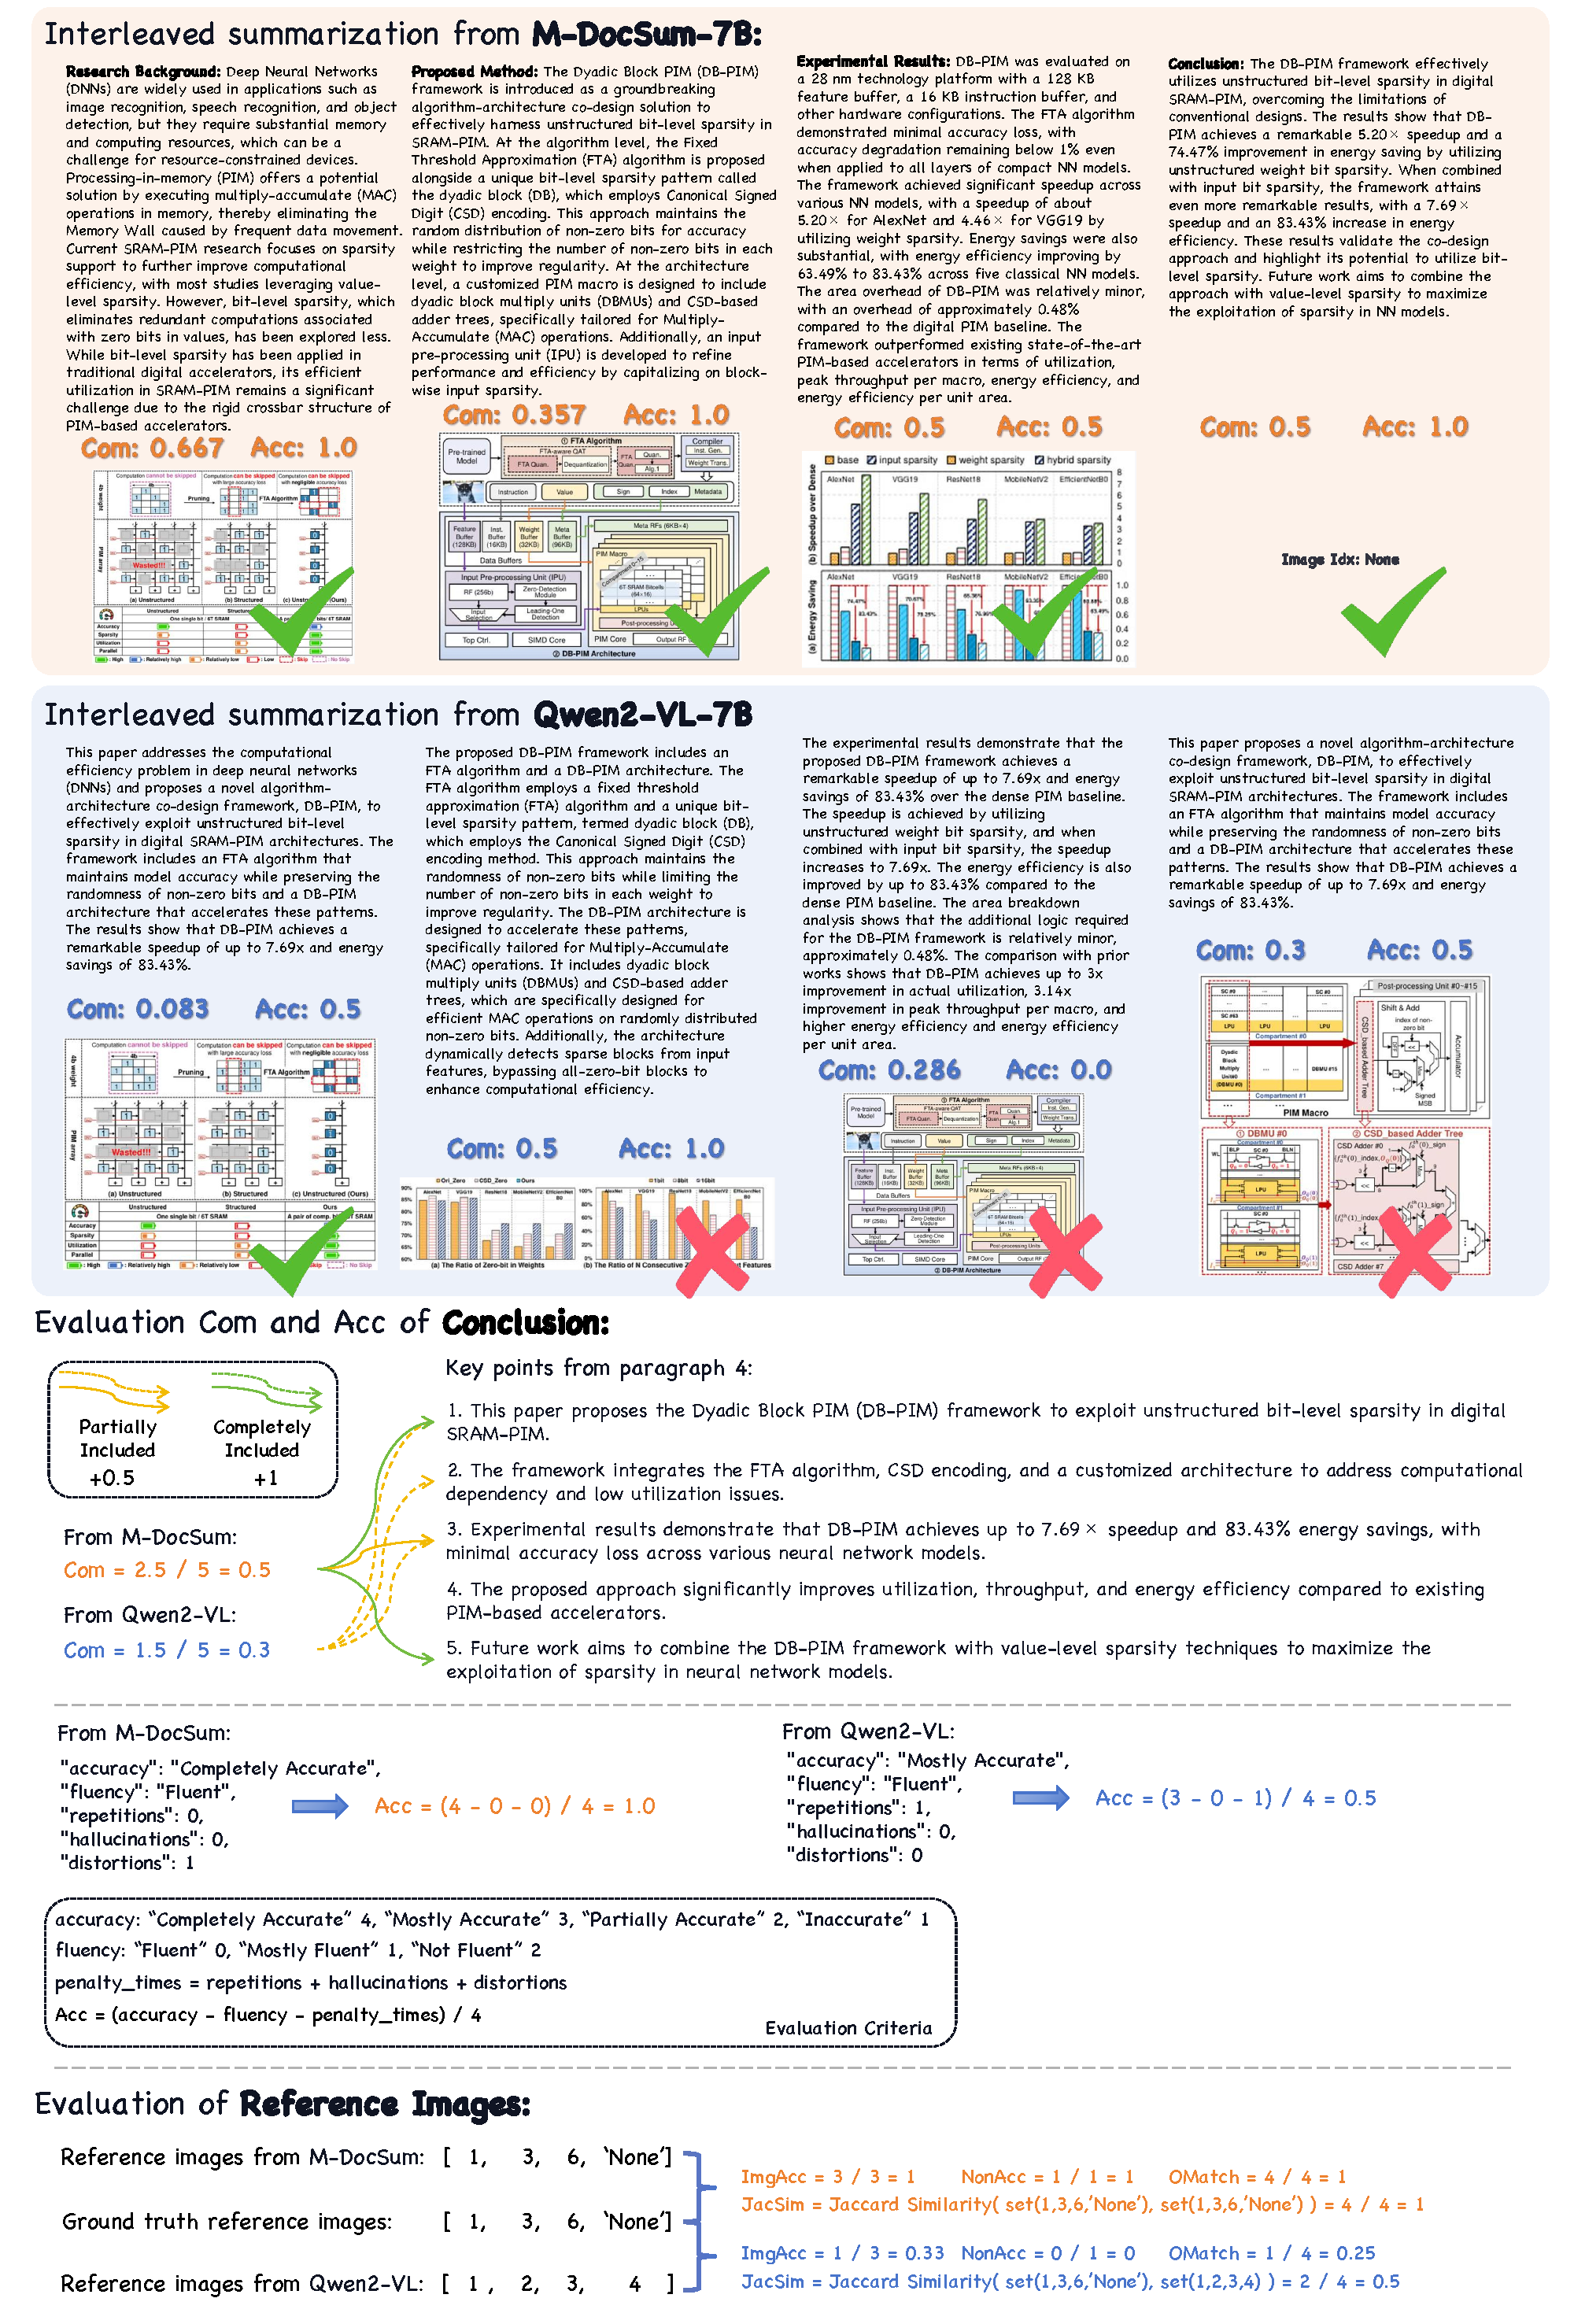
\includegraphics[width=0.77\textwidth]{figs/case_en_2404_09497}
    \captionof{figure}{Presentation 1 of Case Study and M-DocEval Evaluation Methodology.}
    \label{fig:case_en_2}
\end{center}
}]

% \maketitlesupplementary

% \input{ICCV2025-Author-Kit-Feb/tabs/A_prompt_1}

% \begin{figure*}[t]
% \centering
% \includegraphics[width=0.8\textwidth]{ICCV2025-Author-Kit-Feb/figs/case_en_2.pdf}
% \caption{Presentation 1 of Case Study and M-DocEval Evaluation Methodology}
% \label{fig:case_en_2}
% \end{figure*}
\begin{figure*}[t]
\centering
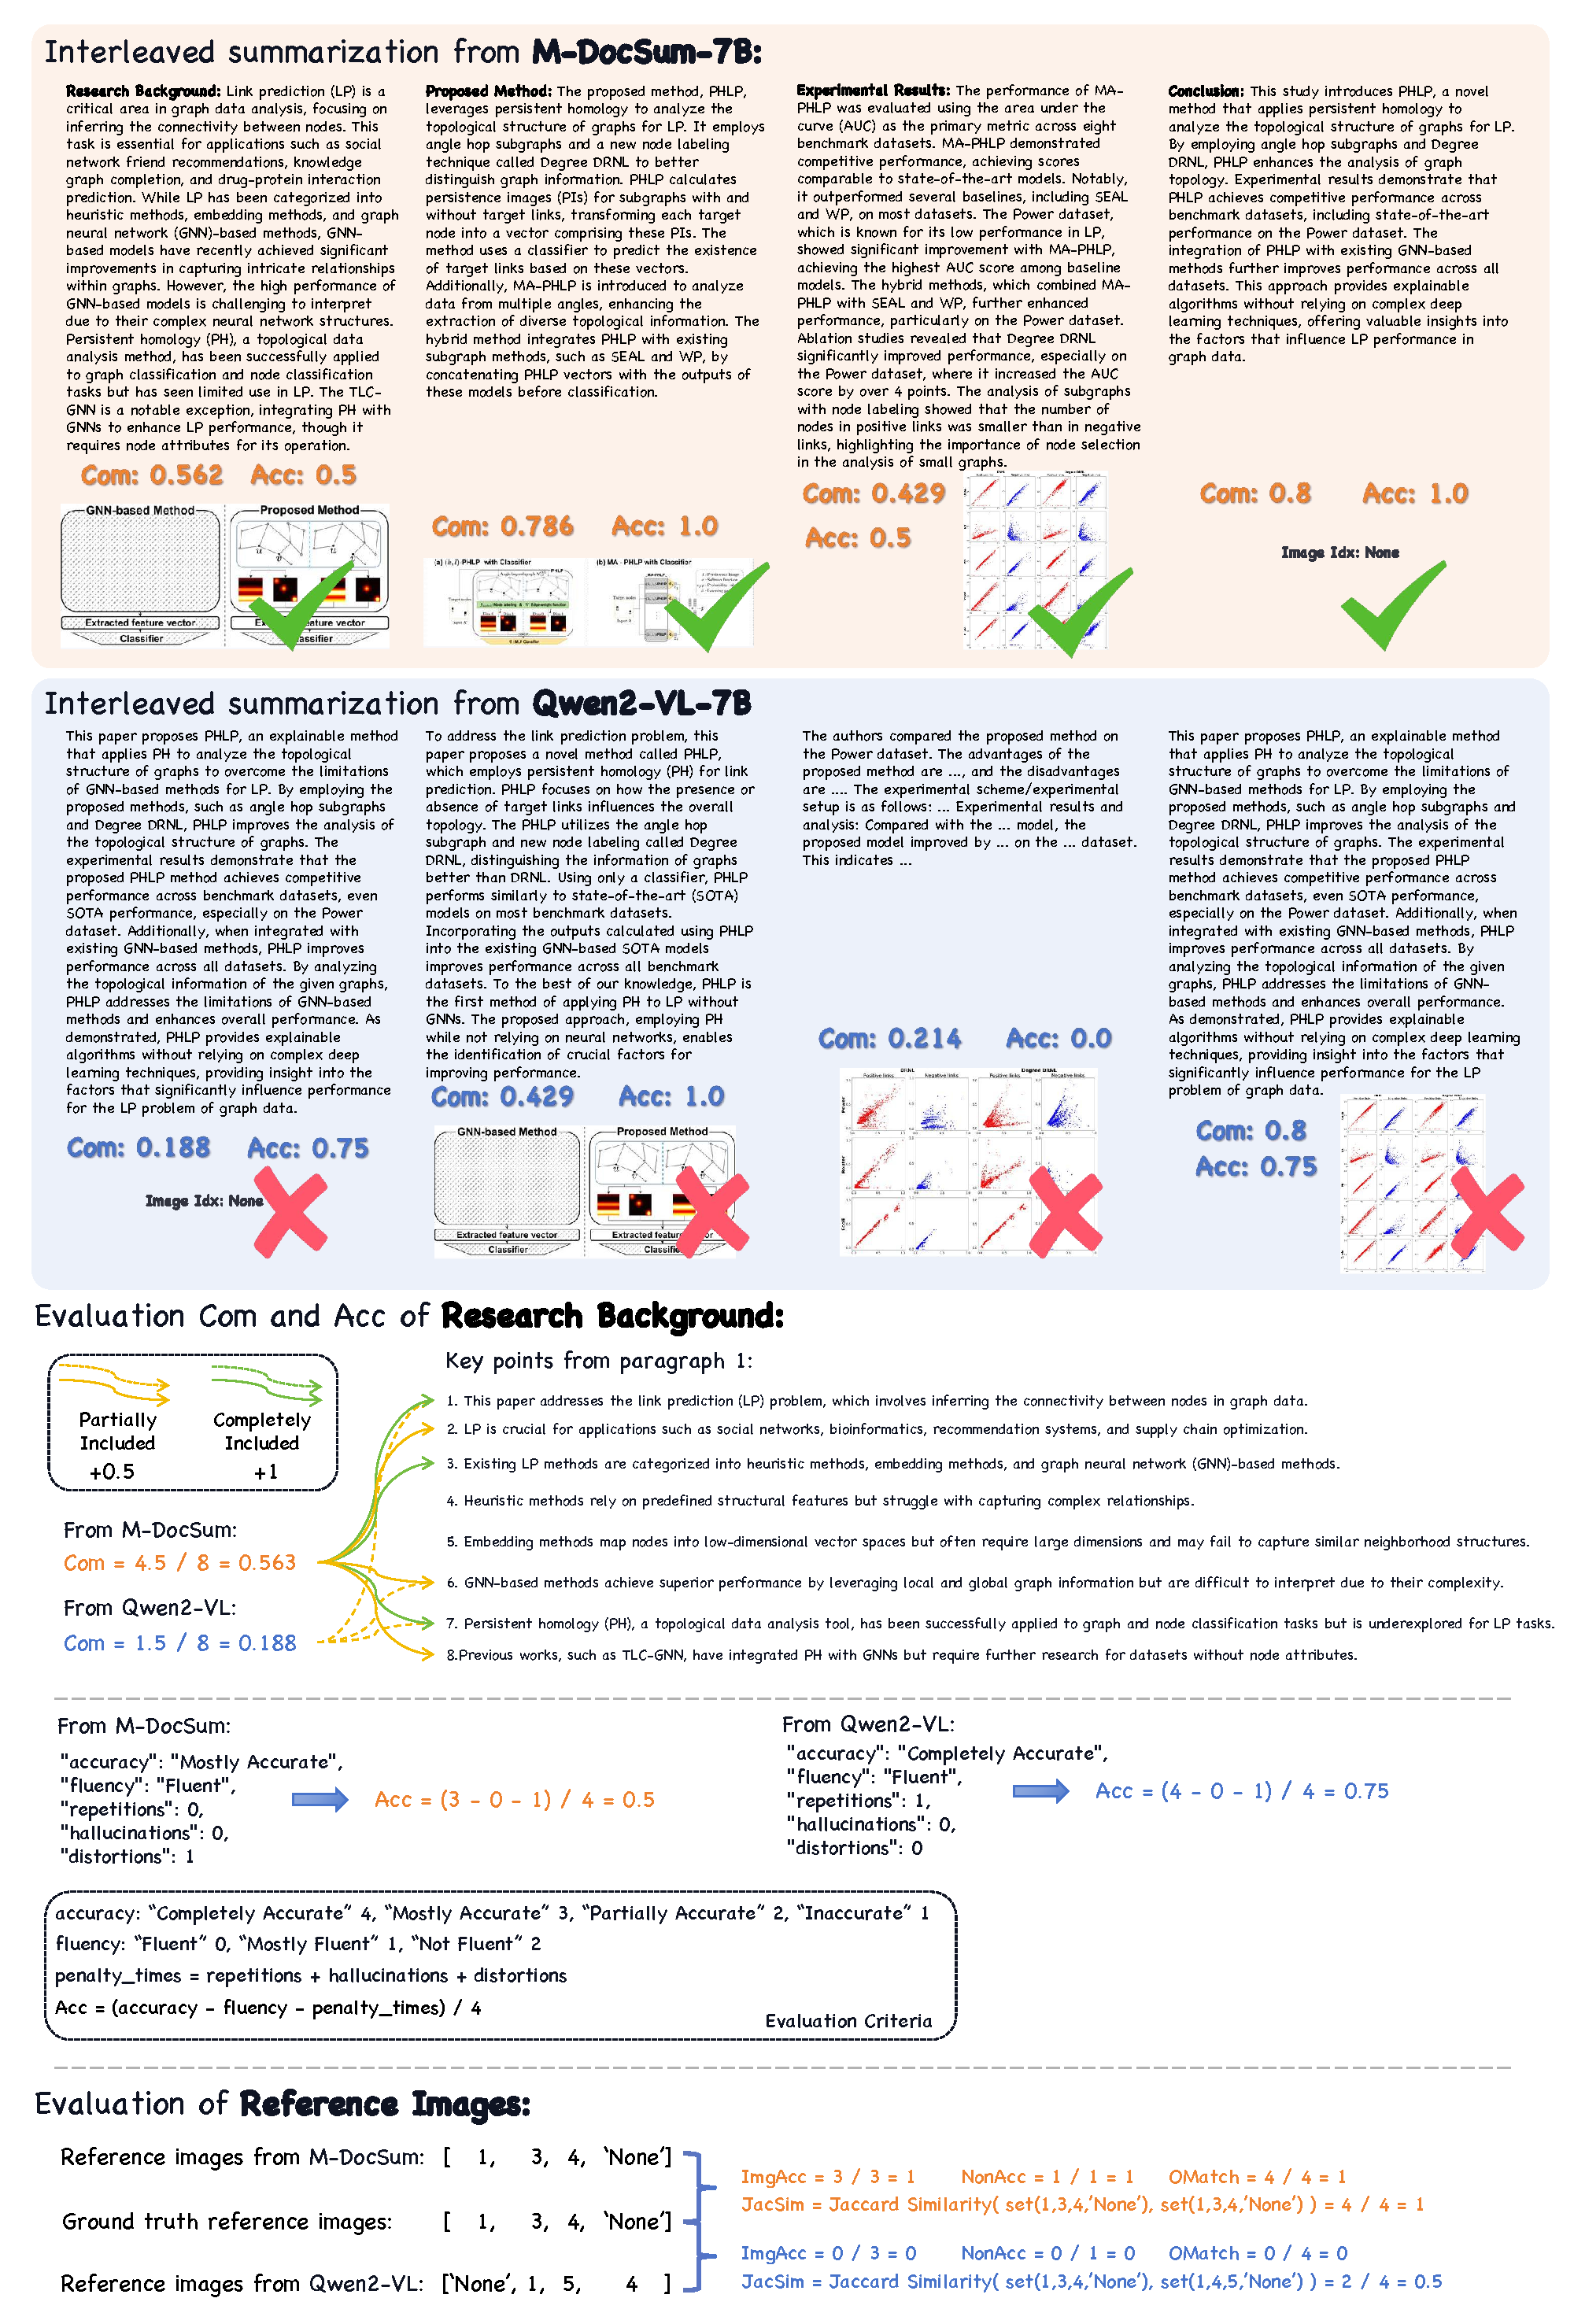
\includegraphics[width=0.8\textwidth]{figs/case_en_2404_15225}
\caption{Presentation 2 of Case Study and M-DocEval Evaluation Methodology}
\label{fig:case_en_1}
\end{figure*}


\twocolumn[{
\renewcommand\twocolumn[1][]{#1}
\section{Prompt Template}
We list the prompt templates used in all processes of the paper, including the automatic data construction, inference, and evaluation stages, in Figures~\ref{fig:prompt1},~\ref{fig:prompt2},~\ref{fig:prompt3},~\ref{fig:prompt_com},~\ref{fig:prompt_acc} and~\ref{fig:prompt_infer}.


% \maketitlesupplementary
\begin{center}
    \centering
    \captionsetup{type=figure}
    \includegraphics[width=0.83\textwidth]{figs/prompt_1}
    \captionof{figure}{Prompt template for key point extraction.}
    \label{fig:prompt1}
\end{center}
}]

% \section{Prompt Template}
% We list the prompt templates used in all processes of the paper, including the automatic data construction, inference, and evaluation stages, in Figures~\ref{fig:prompt1},~\ref{fig:prompt2},~\ref{fig:prompt3},~\ref{fig:prompt_com},~\ref{fig:prompt_acc} and~\ref{fig:prompt_infer}.

% \begin{figure*}[t]
% \centering
% \includegraphics[width=0.9\textwidth]{ICCV2025-Author-Kit-Feb/figs/prompt_1.pdf}
% \caption{Prompt template for key point extraction.}
% \label{fig:prompt1}
% \end{figure*}

\begin{figure*}[t]
\centering
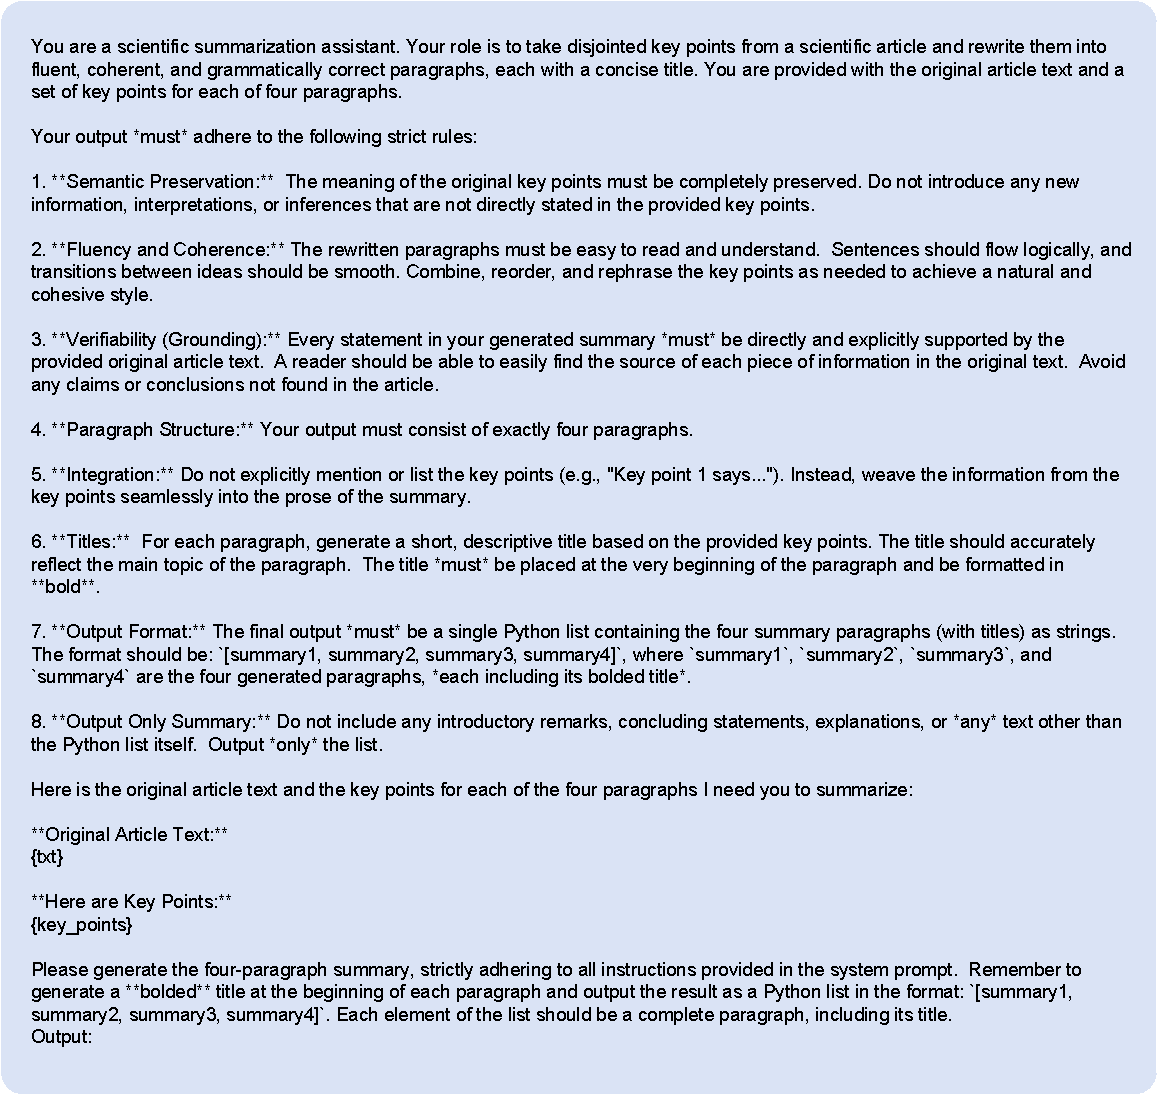
\includegraphics[width=0.9\textwidth]{figs/prompt_2}
\caption{Prompt template for summary generation.}
\label{fig:prompt2}
\end{figure*}

\begin{figure*}[t]
\centering
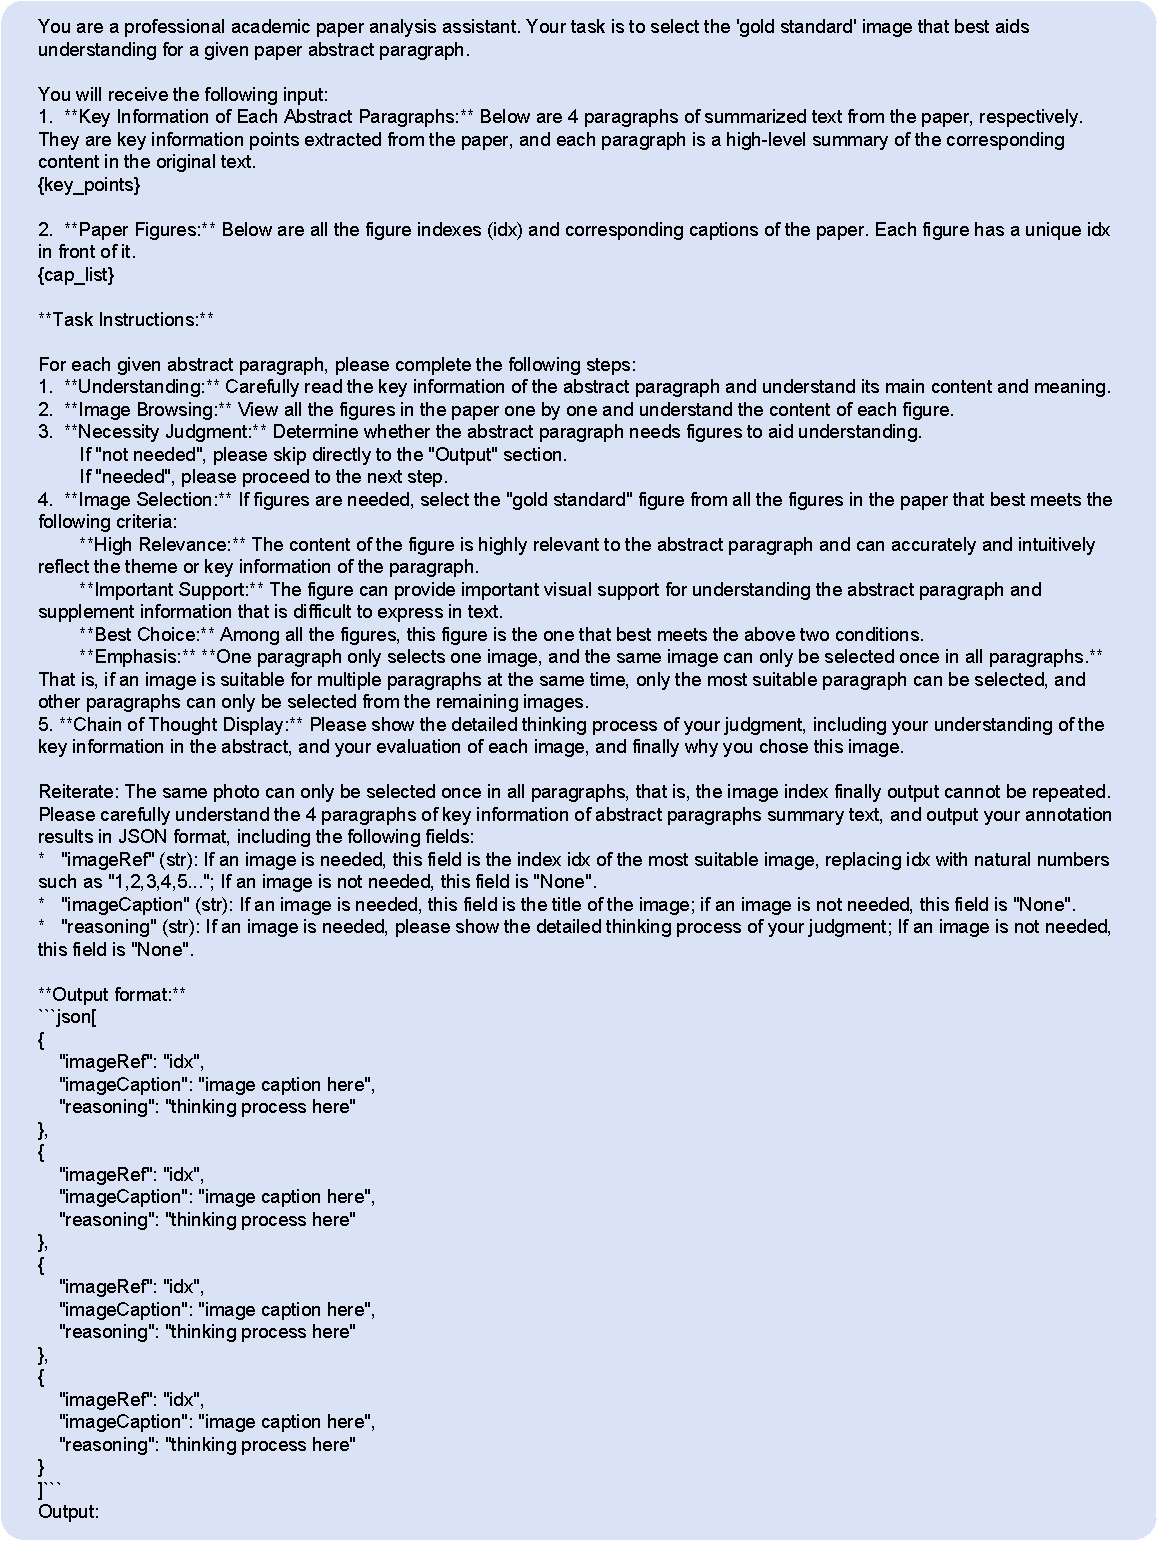
\includegraphics[width=0.9\textwidth]{figs/prompt_3}
\caption{Prompt template for reference image extraction.}
\label{fig:prompt3}
\end{figure*}

\begin{figure*}[t]
\centering
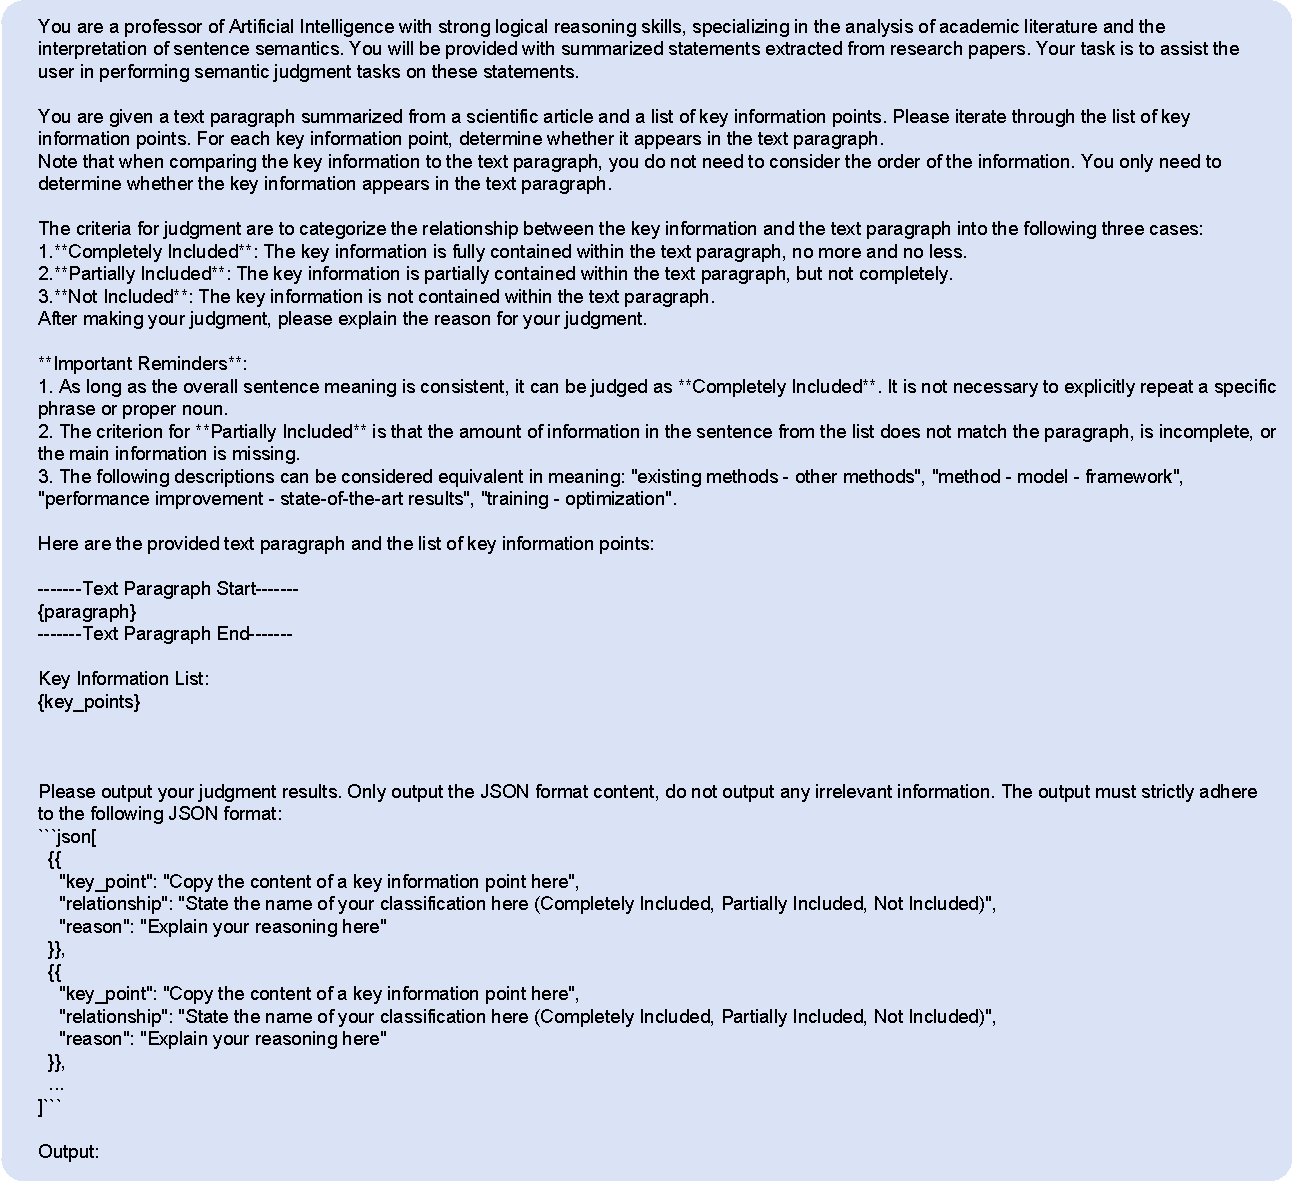
\includegraphics[width=0.9\textwidth]{figs/prompt_com}
\caption{Prompt template for evaluating text Completeness (Com).}
\label{fig:prompt_com}
\end{figure*}

\begin{figure*}[t]
\centering
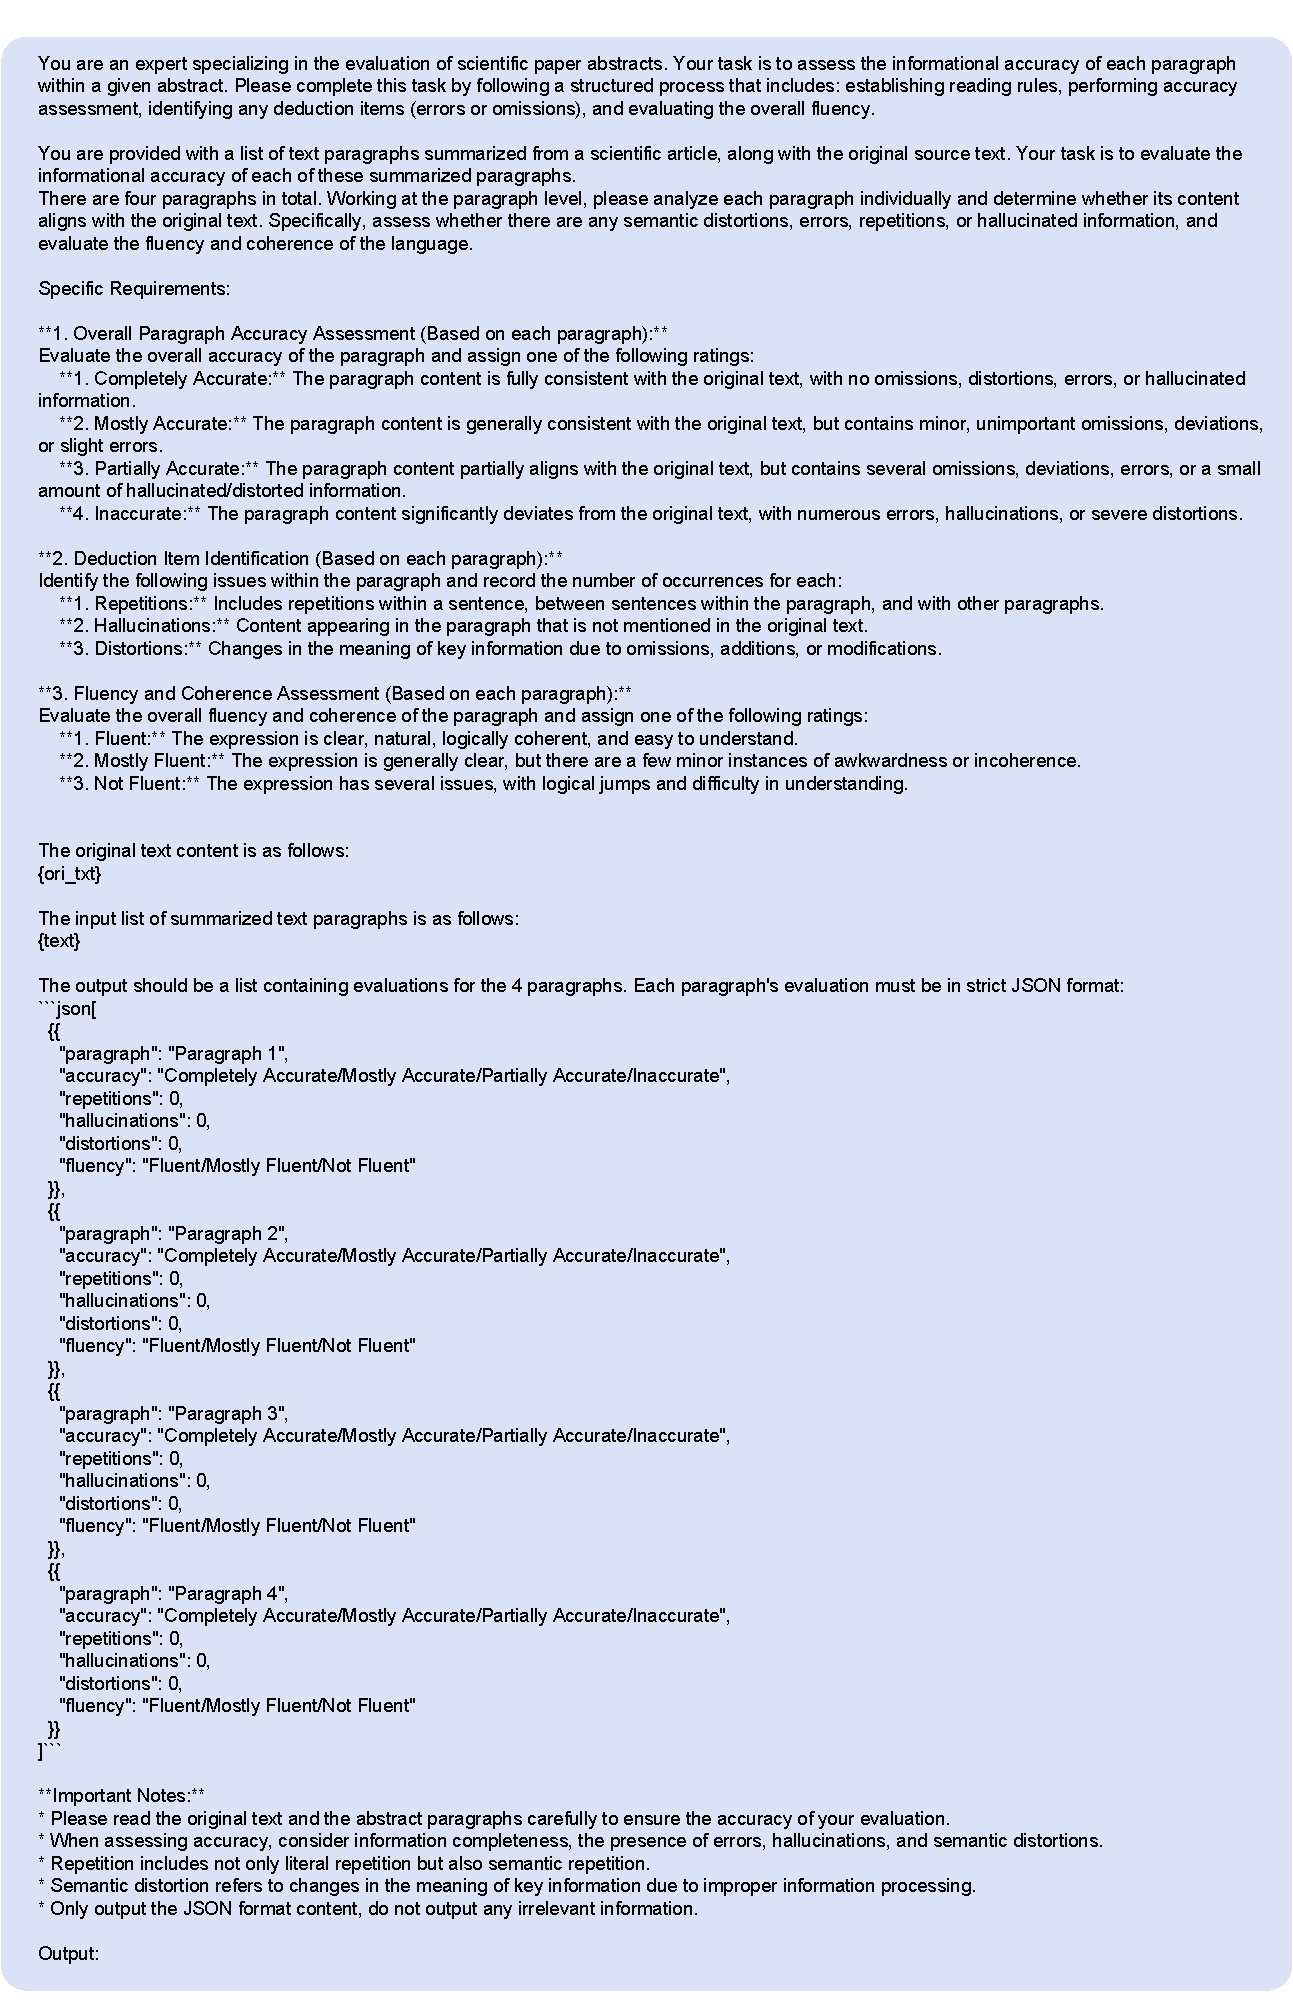
\includegraphics[width=0.8\textwidth]{figs/prompt_acc}
\caption{Prompt template for evaluating text Accuracy (Acc).}
\label{fig:prompt_acc}
\end{figure*}

\begin{figure*}[t]
\centering
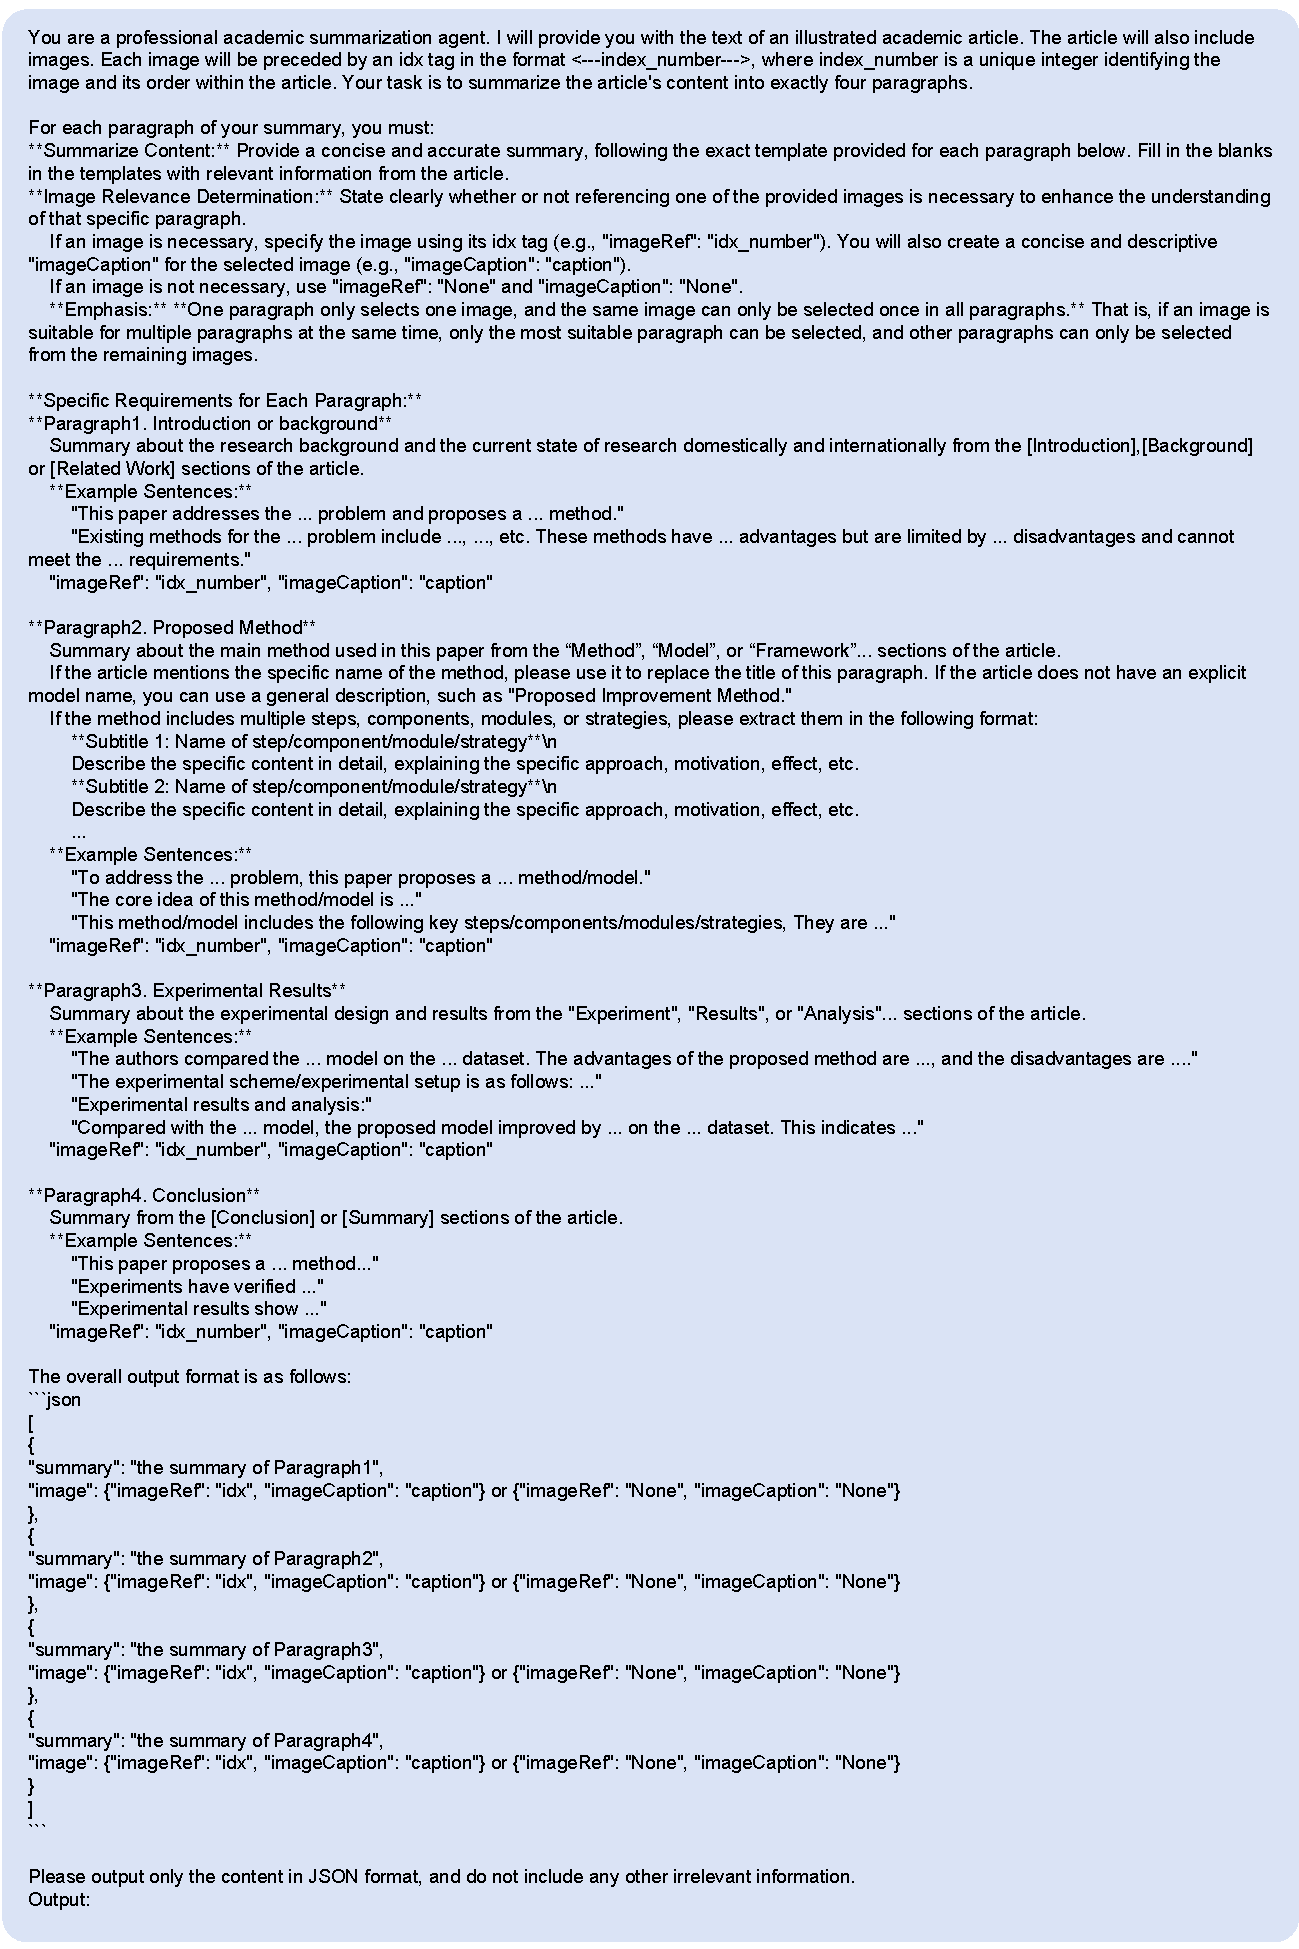
\includegraphics[width=0.8\textwidth]{figs/prompt_6}
\caption{Prompt template for inference.}
\label{fig:prompt_infer}
\end{figure*}

\twocolumn[
\section{Analysis}
\subsection{Paragraph-wise Performance Variations}
\label{Paragraph-wise Performance Variations}
The detailed data in the Table~\ref{tab:para} shows that Gemini Pro, while performing best in summarizing text, maintains only an average level of performance in image referencing. For the Qwen-VL series, upgrading from version 2 to 2.5 results in an overall improvement in text performance, but a varying degree of decline in image referencing is observed.

\subsection{Influence of Context Length on Performance}
\label{Influence of Context Length on Performance}
The detailed data in Table~\ref{tab:token} shows that GPT-4o has a commanding lead in image-related aspects, and Gemini Pro has a commanding lead in text-related aspects, and these leading trends do not diminish as the text length increases. Notably, regarding image referencing capability, the scores of all models decrease by approximately half when the text length increases to 30k compared to the 0-5k range. This is a very pronounced trend.

\subsection{Impact of Image Quantity on Performance}
\label{Impact of Image Quantity on Performance}
From Table~\ref{tab:image}, it is evident that there is a significant difference in the decline of image referencing performance between open-source and closed-source models as the number of images increases. Among the closed-source models, only GPT-4o exhibits a relatively small decline of 9.4\%, while other closed-source models, Claude-3.5 and Gemini-Pro, show declines of 34.4\% and 39.6\%, respectively. Surprisingly, the open-source models Qwen2.5-VL-7B and Qwen2.5-VL-72B experience astonishing declines of 56.6\% and 62.6\%, respectively.

\section{Ablation}
\label{Ablation}
Table~\ref{tab:shuffle} shows that while the robustness of M-DocSum-7B is stronger than that of the base model (+37.5\%) and the model after the first stage of training (+6.8\%), there is still a slight gap compared to powerful closed-source models and larger open-source models. Specifically, the performance after shuffling is lower than that of GPT-4o (-9.4\%), Claude-3.5 (-5.7\%), Gemini Pro (-3.6\%), and Qwen2.5-VL-72B (-1.6\%), indicating that this is an issue worth further investigation in the future.

When we remove the abstract from the original text, the overall performance decline across models is not significant. The largest and smallest declines are observed in Qwen2.5-VL-7B (19.1\%) and M-DocSum-7B (4.5\%), respectively. Notably, the normal score of the model after the first stage of training is higher than that of M-DocSum-7B by 2.4\%, but its performance after removing the abstract is lower by 1.6\%. This provides strong evidence that the second stage of training enhances the model's robustness.
]




\begin{table*}[t]
\caption{TS and OMatch Across Different Models and Paragraphs}
\centering
\resizebox{0.85\textwidth}{!}{
\begin{tabular}{l|cc|cc|cc|cc}
\toprule
\multirow{2}{*}{Model} & \multicolumn{2}{c|}{para 1} & \multicolumn{2}{c|}{para 2} & \multicolumn{2}{c|}{para 3} & \multicolumn{2}{c}{para 4} \\
\cmidrule(lr){2-3} \cmidrule(lr){4-5} \cmidrule(lr){6-7} \cmidrule(lr){8-9}
 & TS & OMatch & TS & OMatch & TS & OMatch & TS & OMatch \\
\midrule
GPT-4o & 0.596 & 0.705 & 0.637 & 0.531 & 0.560 & 0.489 & 0.610 & 0.571 \\
Gemini-Pro & 0.670 & 0.547 & 0.705 & 0.421 & 0.647 & 0.477 & 0.722 & 0.419 \\
Claude-3-5-Sonnet & 0.623 & 0.628 & 0.658 & 0.458 & 0.589 & 0.496 & 0.685 & 0.448 \\
Qwen2.5-VL-72B & 0.536 & 0.263 & 0.568 & 0.208 & 0.542 & 0.288 & 0.588 & 0.512 \\
Qwen2-VL-72B & 0.475 & 0.447 & 0.586 & 0.372 & 0.438 & 0.423 & 0.485 & 0.600 \\
Qwen2.5-VL-7B & 0.497 & 0.255 & 0.558 & 0.121 & 0.472 & 0.157 & 0.533 & 0.570 \\
Qwen2-VL-7B & 0.433 & 0.518 & 0.498 & 0.293 & 0.375 & 0.214 & 0.479 & 0.194 \\

\bottomrule
\end{tabular}
}
\label{tab:para}
\end{table*}

\begin{table*}[t]
\caption{TS and OMatch Across Different Models and Token Length}
\centering
\resizebox{0.95\textwidth}{!}{
\begin{tabular}{l|cc|cc|cc|cc|cc|cc}
\toprule
\multirow{2}{*}{Model} & \multicolumn{2}{c|}{0\textasciitilde5k} & \multicolumn{2}{c|}{5\textasciitilde10k} & \multicolumn{2}{c|}{10\textasciitilde15k} & \multicolumn{2}{c|}{15\textasciitilde20k} & \multicolumn{2}{c|}{20\textasciitilde25k} & \multicolumn{2}{c}{25\textasciitilde30k} \\
\cmidrule(lr){2-3} \cmidrule(lr){4-5} \cmidrule(lr){6-7} \cmidrule(lr){8-9} \cmidrule(lr){10-11} \cmidrule(lr){12-13}
 & TS & OMatch & TS & OMatch & TS & OMatch & TS & OMatch & TS & OMatch & TS & OMatch \\
\midrule
GPT-4o & 0.594 & 0.688 & 0.605 & 0.547 & 0.608 & 0.514 & 0.600 & 0.552 & 0.621 & 0.381 & 0.609 & 0.414 \\
Gemini-Pro & 0.687 & 0.585 & 0.688 & 0.468 & 0.694 & 0.366 & 0.673 & 0.401 & 0.688 & 0.298 & 0.668 & 0.283 \\
Claude-3-5-Sonnet & 0.630 & 0.646 & 0.643 & 0.464 & 0.655 & 0.458 & 0.623 & 0.453 & 0.662 & 0.333 & 0.645 & 0.329 \\
Qwen2.5-VL-72B & 0.544 & 0.463 & 0.561 & 0.260 & 0.559 & 0.218 & 0.552 & 0.234 & 0.543 & 0.155 & 0.517 & 0.211 \\
Qwen2-VL-72B & 0.499 & 0.604 & 0.503 & 0.456 & 0.514 & 0.377 & 0.464 & 0.302 & 0.490 & 0.286 & 0.467 & 0.257 \\
Qwen2.5-VL-7B & 0.495 & 0.397 & 0.477 & 0.185 & 0.412 & 0.158 & 0.423 & 0.156 & 0.412 & 0.107 & 0.428 & 0.184 \\
Qwen2-VL-7B & 0.444 & 0.350 & 0.449 & 0.299 & 0.430 & 0.275 & 0.404 & 0.224 & 0.442 & 0.250 & 0.389 & 0.197 \\

\bottomrule
\end{tabular}
}
\label{tab:token}
\end{table*}
\begin{table*}[h]
\caption{TS and OMatch Across Different Models and Image Numbers}
\centering
\resizebox{0.95\textwidth}{!}{
\begin{tabular}{l|cc|cc|cc|cc|cc|cc}
\toprule
\multirow{2}{*}{Model} & \multicolumn{2}{c|}{1\textasciitilde3} & \multicolumn{2}{c|}{4\textasciitilde6} & \multicolumn{2}{c|}{7\textasciitilde9} & \multicolumn{2}{c|}{10\textasciitilde12} & \multicolumn{2}{c|}{13\textasciitilde15} & \multicolumn{2}{c}{16\textasciitilde17} \\
\cmidrule(lr){2-3} \cmidrule(lr){4-5} \cmidrule(lr){6-7} \cmidrule(lr){8-9} \cmidrule(lr){10-11} \cmidrule(lr){12-13}
 & TS & OMatch & TS & OMatch & TS & OMatch & TS & OMatch & TS & OMatch & TS & OMatch \\
\midrule
GPT-4o & 0.567 & 0.540 & 0.613 & 0.616 & 0.613 & 0.562 & 0.605 & 0.535 & 0.559 & 0.591 & 0.550 & 0.489 \\
Gemini-Pro & 0.670 & 0.540 & 0.692 & 0.520 & 0.696 & 0.441 & 0.678 & 0.459 & 0.658 & 0.392 & 0.667 & 0.326 \\
Claude-3-5-Sonnet & 0.618 & 0.680 & 0.636 & 0.534 & 0.640 & 0.486 & 0.650 & 0.485 & 0.634 & 0.466 & 0.645 & 0.446 \\
Qwen2.5-VL-72B & 0.573 & 0.590 & 0.562 & 0.347 & 0.560 & 0.256 & 0.534 & 0.276 & 0.519 & 0.278 & 0.494 & 0.337 \\
Qwen2-VL-72B & 0.520 & 0.520 & 0.516 & 0.519 & 0.505 & 0.438 & 0.473 & 0.429 & 0.467 & 0.352 & 0.411 & 0.402 \\
Qwen2.5-VL-7B & 0.511 & 0.500 & 0.481 & 0.301 & 0.479 & 0.203 & 0.461 & 0.197 & 0.382 & 0.188 & 0.315 & 0.185 \\
Qwen2-VL-7B & 0.431 & 0.320 & 0.434 & 0.346 & 0.459 & 0.278 & 0.420 & 0.279 & 0.412 & 0.233 & 0.388 & 0.217 \\

\bottomrule
\end{tabular}
}
\label{tab:image}
\end{table*}

% \section{Paragraph-wise Performance Variations}

% 
\begin{table*}[t]
\caption{TS and OMatch Across Different Models and Paragraphs}
\centering
\resizebox{0.85\textwidth}{!}{
\begin{tabular}{l|cc|cc|cc|cc}
\toprule
\multirow{2}{*}{Model} & \multicolumn{2}{c|}{para 1} & \multicolumn{2}{c|}{para 2} & \multicolumn{2}{c|}{para 3} & \multicolumn{2}{c}{para 4} \\
\cmidrule(lr){2-3} \cmidrule(lr){4-5} \cmidrule(lr){6-7} \cmidrule(lr){8-9}
 & TS & OMatch & TS & OMatch & TS & OMatch & TS & OMatch \\
\midrule
GPT-4o & 0.596 & 0.705 & 0.637 & 0.531 & 0.560 & 0.489 & 0.610 & 0.571 \\
Gemini-Pro & 0.670 & 0.547 & 0.705 & 0.421 & 0.647 & 0.477 & 0.722 & 0.419 \\
Claude-3-5-Sonnet & 0.623 & 0.628 & 0.658 & 0.458 & 0.589 & 0.496 & 0.685 & 0.448 \\
Qwen2.5-VL-72B & 0.536 & 0.263 & 0.568 & 0.208 & 0.542 & 0.288 & 0.588 & 0.512 \\
Qwen2-VL-72B & 0.475 & 0.447 & 0.586 & 0.372 & 0.438 & 0.423 & 0.485 & 0.600 \\
Qwen2.5-VL-7B & 0.497 & 0.255 & 0.558 & 0.121 & 0.472 & 0.157 & 0.533 & 0.570 \\
Qwen2-VL-7B & 0.433 & 0.518 & 0.498 & 0.293 & 0.375 & 0.214 & 0.479 & 0.194 \\

\bottomrule
\end{tabular}
}
\label{tab:para}
\end{table*}



% \begin{table*}[h]
\caption{Comparison with Image Score and Decline Rates}
\centering
\resizebox{0.45\textwidth}{!}{
\begin{tabular}{lcc}
\toprule
Models                      & Original IS & Shuffled IS \\
\midrule
GPT-4o                   & 0.638          & 0.533           \\
Gemini-pro                 & 0.553          & 0.501           \\
Claude-3-5-sonnet & 0.589          & 0.512           \\
Qwen2.5-VL-72B             & 0.517          & 0.491           \\
Qwen2-vl-72B               & 0.485          & 0.399           \\
Qwen2.5-vl-7B               & 0.423          & 0.373           \\
Qwen2-vl-7B                & 0.421          & 0.302           \\
Stage-1       & 0.615          & 0.450           \\
M-DocSum-7B      & 0.636          & 0.483           \\
M-DocSum-7B w/o stage-1                 & 0.556          & 0.405         \\
\bottomrule
\end{tabular}
}
\label{tab:shuffle}
\end{table*}

% \begin{table*}[h]
\caption{Comparison with Text Score and Decline Rates}
\centering
\resizebox{0.45\textwidth}{!}{
\begin{tabular}{lcc}
\toprule
Models                     & Original TS & W/o abstract TS \\
\midrule
Qwen2.5-VL-7B                       & 0.517	&0.418           \\
Qwen2-VL-7B         &  0.449&	0.402           \\
InternVL2-8B & 0.513&	0.435          \\
InternVL2.5-8B             & 0.529&	0.488           \\
Stage-1                & 0.660&	0.605          \\
M-DocSum-7B               & 0.644&	0.615         \\

\bottomrule
\end{tabular}
}
\label{tab:abs}
\end{table*}

\begin{table*}[t] % Use [t] to place at the top of the next page if necessary
\centering
% \caption{Performance Comparisons under Different Conditions} % Overall caption
\begin{minipage}{0.4\textwidth}
  \centering
  \caption{Image Score and Decline Rates (Shuffled)} % Sub-caption
  \resizebox{\textwidth}{!}{
    \begin{tabular}{lcc}
    \toprule
    Models                      & Original IS & Shuffled IS \\
    \midrule
    GPT-4o                   & 0.638          & 0.533           \\
    Gemini-pro                 & 0.553          & 0.501           \\
    Claude-3-5-sonnet & 0.589          & 0.512           \\
    Qwen2.5-VL-72B             & 0.517          & 0.491           \\
    Qwen2-vl-72B               & 0.485          & 0.399           \\
    Qwen2.5-vl-7B               & 0.423          & 0.373           \\
    Qwen2-vl-7B                & 0.421          & 0.302           \\
    Stage-1       & 0.615          & 0.450           \\
    M-DocSum-7B      & 0.636          & 0.483           \\
    M-DocSum-7B w/o stage-1                 & 0.556          & 0.405         \\
    \bottomrule
    \end{tabular}
  }
  \label{tab:shuffle}
\end{minipage}\hspace{0.05\textwidth}
\begin{minipage}{0.4\textwidth}
  \centering
  \caption{Text Score and Decline Rates (W/o Abstract)} % Sub-caption
  \resizebox{\textwidth}{!}{
    \begin{tabular}{lcc}
    \toprule
    Models                     & Original TS & W/o abstract TS \\
    \midrule
    Qwen2.5-VL-7B                       & 0.517	&0.418           \\
    Qwen2-VL-7B         &  0.449&	0.402           \\
    InternVL2-8B & 0.513&	0.435          \\
    InternVL2.5-8B             & 0.529&	0.488           \\
    Stage-1                & 0.660&	0.605          \\
    M-DocSum-7B               & 0.644&	0.615         \\
    \bottomrule
    \end{tabular}
  }
  \label{tab:abs}
\end{minipage}
\end{table*}


% \section{Rationale}
% \label{sec:rationale}

% \begin{table*}[h]
% \centering
% \caption{Overall Results.}
% \begin{tabular}{|l|c|c|c|c|c|c|c|c|c|c|c|c|c|c|}
% \hline
% \multirow{2}{*}{Models} & \multirow{2}{*}{Frames} & \multirow{2}{*}{Overall} & \multicolumn{3}{|c|}{Cognitive} & \multicolumn{3}{|c|}{Temporal Event}  \\ \cline{4-9} 
% & & &Perception & Understanding & Reasoning & low & mid & high  \\ \hline
%  \multicolumn{9}{|c|}{Proprietary Models} \\ \hline
% Human & 8frames & 45.8 & 45.0 & 46.28 & 46.26 & 100 & 12.91 & 17.45   \\ \hline 
% Human & 1fps & 63.6 & 67.6 & 63.2 & 59.34 & 100 & 100 & 18.6   \\ \hline
% Human & 8fps & 80.3 & 94.66 & 75.0 & 71.96 & 84.72 & 86.42 & 70.1   \\ \hline
% GPT-4o & 8 & 41.07 & 26.31 & 41.38 & 48.61 & 54.0 & 32.61 & 37.5   \\ \hline 
% GPT-4o & 16 & 45.23 & 31.58 & 51.72 & 47.2 & 68.0 & 36.96 & 34.72   \\ \hline
% GPT-4o & 32 & 47.02 & 28.95 & 63.79 & 43.56 & 50.0 & 43.48 & 47.22   \\ \hline
% GPT-4o & 64 & 42.26 & 18.4 & 50.0 & 48.6 & 58.0 & 23.9 & 43.05   \\ \hline
% \end{tabular}
% \end{table*}

% Having the supplementary compiled together with the main paper means that:
% % 
% \begin{itemize}
% \item The supplementary can back-reference sections of the main paper, for example, we can refer to \cref{sec:intro};
% \item The main paper can forward reference sub-sections within the supplementary explicitly (e.g. referring to a particular experiment); 
% \item When submitted to arXiv, the supplementary will already included at the end of the paper.
% \end{itemize}
% % 
% To split the supplementary pages from the main paper, you can use \href{https://support.apple.com/en-ca/guide/preview/prvw11793/mac#:~:text=Delete%20a%20page%20from%20a,or%20choose%20Edit%20%3E%20Delete).}{Preview (on macOS)}, \href{https://www.adobe.com/acrobat/how-to/delete-pages-from-pdf.html#:~:text=Choose%20%E2%80%9CTools%E2%80%9D%20%3E%20%E2%80%9COrganize,or%20pages%20from%20the%20file.}{Adobe Acrobat} (on all OSs), as well as \href{https://superuser.com/questions/517986/is-it-possible-to-delete-some-pages-of-a-pdf-document}{command line tools}.

% \section{Existing Benchmark}


% \section{Benchmark Details}
% \subsection{Answer Evaluation Prompt}
% \begin{tcolorbox}[colframe=black, colback=gray!10, coltitle=white, title=\textbf{Answer Evaluation Prompt}]
% \label{evaluation_prompt}
% You are an \textbf{impartial evaluator}, and you have been assigned a scoring task. You will receive a description of a video, a question related to the video, the corresponding correct answer (gt), and an answer provided by a video language model for the same question. Your task is to compare the model's answer with the correct answer and assign a score.

% The \textbf{scoring rules }are as follows:

% The score range is 0, 1, or 2. The video description serves as auxiliary information to help you determine whether the model's answer accurately reflects the content of the video.
% When the model's answer matches the meaning of the correct answer completely, give 2 points. (TWO EXAMPLES)\\
% Note that the exact words do not need to be the same, as 
% long as the meaning conveyed is the same.
% When the model's answer partially matches the correct answer and does not contain any conflicting information, give 1 point. (TWO EXAMPLES)\\
% If the model's answer completely contradicts the correct answer, give 0 points. (TWO EXAMPLES)\\
% Please carefully evaluate the model's answer according to the above criteria to ensure fairness and consistency in scoring.

% \textbf{Question}: {}\\
% Video Description: {}\\
% Correct Answer: {}\\
% Model's Answer: {}\\

% Your \textbf{score format} is as follows:\\
% Reasoning: REASON \\
% Therefore, the model's score is: SCORE
% \end{tcolorbox}

